\chapter{M\'odulo de Vacunaci\'on}

\section{Descripci\'on General}

El m\'odulo de vacunaci\'on consta de dos partes: un cat\'alogo de vacunas
(\texttt{vaccines}) y los registros de aplicaci\'on
(\texttt{vaccination\_records}). Permite el seguimiento completo del
esquema de vacunaci\'on de cada paciente.

\section{Cat\'alogo de Vacunas}

Cada vacuna en el cat\'alogo tiene:

\begin{itemize}[leftmargin=*]
    \item Nombre y descripci\'on.
    \item Especie objetivo (dog, cat, rabbit, bird, etc.).
    \item Frecuencia en d\'{\i}as (por defecto 365).
    \item Indicador de vacuna esencial (core).
\end{itemize}

\section{Registros de Vacunaci\'on}

Cada aplicaci\'on registra:

\begin{itemize}[leftmargin=*]
    \item Paciente y vacuna aplicada.
    \item Fecha de aplicaci\'on y pr\'oxima fecha de refuerzo.
    \item N\'umero de lote y sitio de aplicaci\'on.
    \item N\'umero de dosis.
    \item Profesional que administr\'o.
\end{itemize}

\section{Server Actions}

\subsection{getVaccinations --- Dos Modos de Consulta}

\begin{lstlisting}[style=typescript, caption=Vacunacion - Dos modos de consulta]
// Modo 1: Detalle por paciente (cached)
const getVaccinationsByPatient = cache(
  async (patientId: number): Promise<VaccinationWithDetails[]> => {
    const rows = await db
      .select({
        id: schema.vaccinationRecords.id,
        patientId: schema.vaccinationRecords.patientId,
        vaccineId: schema.vaccinationRecords.vaccineId,
        vaccineName: schema.vaccines.name,
        appliedDate: schema.vaccinationRecords.appliedDate,
        nextDueDate: schema.vaccinationRecords.nextDueDate,
        batchNumber: schema.vaccinationRecords.batchNumber,
        applicationSite: schema.vaccinationRecords.applicationSite,
        doseNumber: schema.vaccinationRecords.doseNumber,
        administeredByName: sql`CONCAT(${schema.users.firstName},
                                ' ', ${schema.users.lastName})`,
      })
      .from(schema.vaccinationRecords)
      .innerJoin(schema.patients,
        eq(schema.patients.id, schema.vaccinationRecords.patientId))
      .innerJoin(schema.clients,
        eq(schema.clients.id, schema.patients.clientId))
      .innerJoin(schema.vaccines,
        eq(schema.vaccines.id, schema.vaccinationRecords.vaccineId))
      .leftJoin(schema.users,
        eq(schema.users.id, schema.vaccinationRecords.administeredBy))
      .where(eq(schema.vaccinationRecords.patientId, patientId))
      .orderBy(desc(schema.vaccinationRecords.appliedDate));

    return rows.map((r) => ({
      ...r,
      appliedDate: String(r.appliedDate).split('T')[0],
      nextDueDate: r.nextDueDate
        ? String(r.nextDueDate).split('T')[0] : null,
    }));
  }
);

// Modo 2: Resumen por paciente (agregado)
export async function getVaccinations(
  patientId?: number
): Promise<VaccinationWithDetails[] | PatientVaccinationSummary[]> {
  if (patientId) {
    return getVaccinationsByPatient(patientId);
  }

  // Agregacion: ultima vacuna, proxima dosis, conteo
  const rows = await db
    .select({
      patientId: schema.patients.id,
      patientName: schema.patients.name,
      patientSpecies: schema.patients.species,
      clientName: schema.clients.name,
      lastVaccineDate:
        sql<string | null>`max(${schema.vaccinationRecords.appliedDate})`,
      nextDueDate:
        sql<string | null>`min(${schema.vaccinationRecords.nextDueDate})`,
      vaccineCount:
        sql<number>`count(${schema.vaccinationRecords.id})::int`,
    })
    .from(schema.patients)
    .innerJoin(schema.clients,
      eq(schema.clients.id, schema.patients.clientId))
    .leftJoin(schema.vaccinationRecords,
      eq(schema.vaccinationRecords.patientId, schema.patients.id))
    .where(and(eq(schema.patients.clinicId, clinicId),
               eq(schema.patients.active, true)))
    .groupBy(schema.patients.id, schema.clients.id)
    .orderBy(schema.patients.name);

  return rows;
}
\end{lstlisting}

\subsection{Caracter\'isticas Destacadas}

\begin{itemize}[leftmargin=*]
    \item \textbf{React cache():} La funci\'on de detalle por paciente usa
          \texttt{cache()} de React para deduplicaci\'on de llamadas.
    \item \textbf{Dos modos:} Detalle completo (por paciente) y resumen
          agregado (todos los pacientes de la cl\'{\i}nica).
    \item \textbf{SQL raw:} Usa \texttt{sql} template literal para funciones
          de agregaci\'on como \texttt{MAX}, \texttt{MIN}, \texttt{COUNT}.
    \item \textbf{Formato de fechas:} Las fechas se truncan a
          \texttt{YYYY-MM-DD} eliminando el componente de hora.
\end{itemize}

\begin{figure}[H]
    \centering
    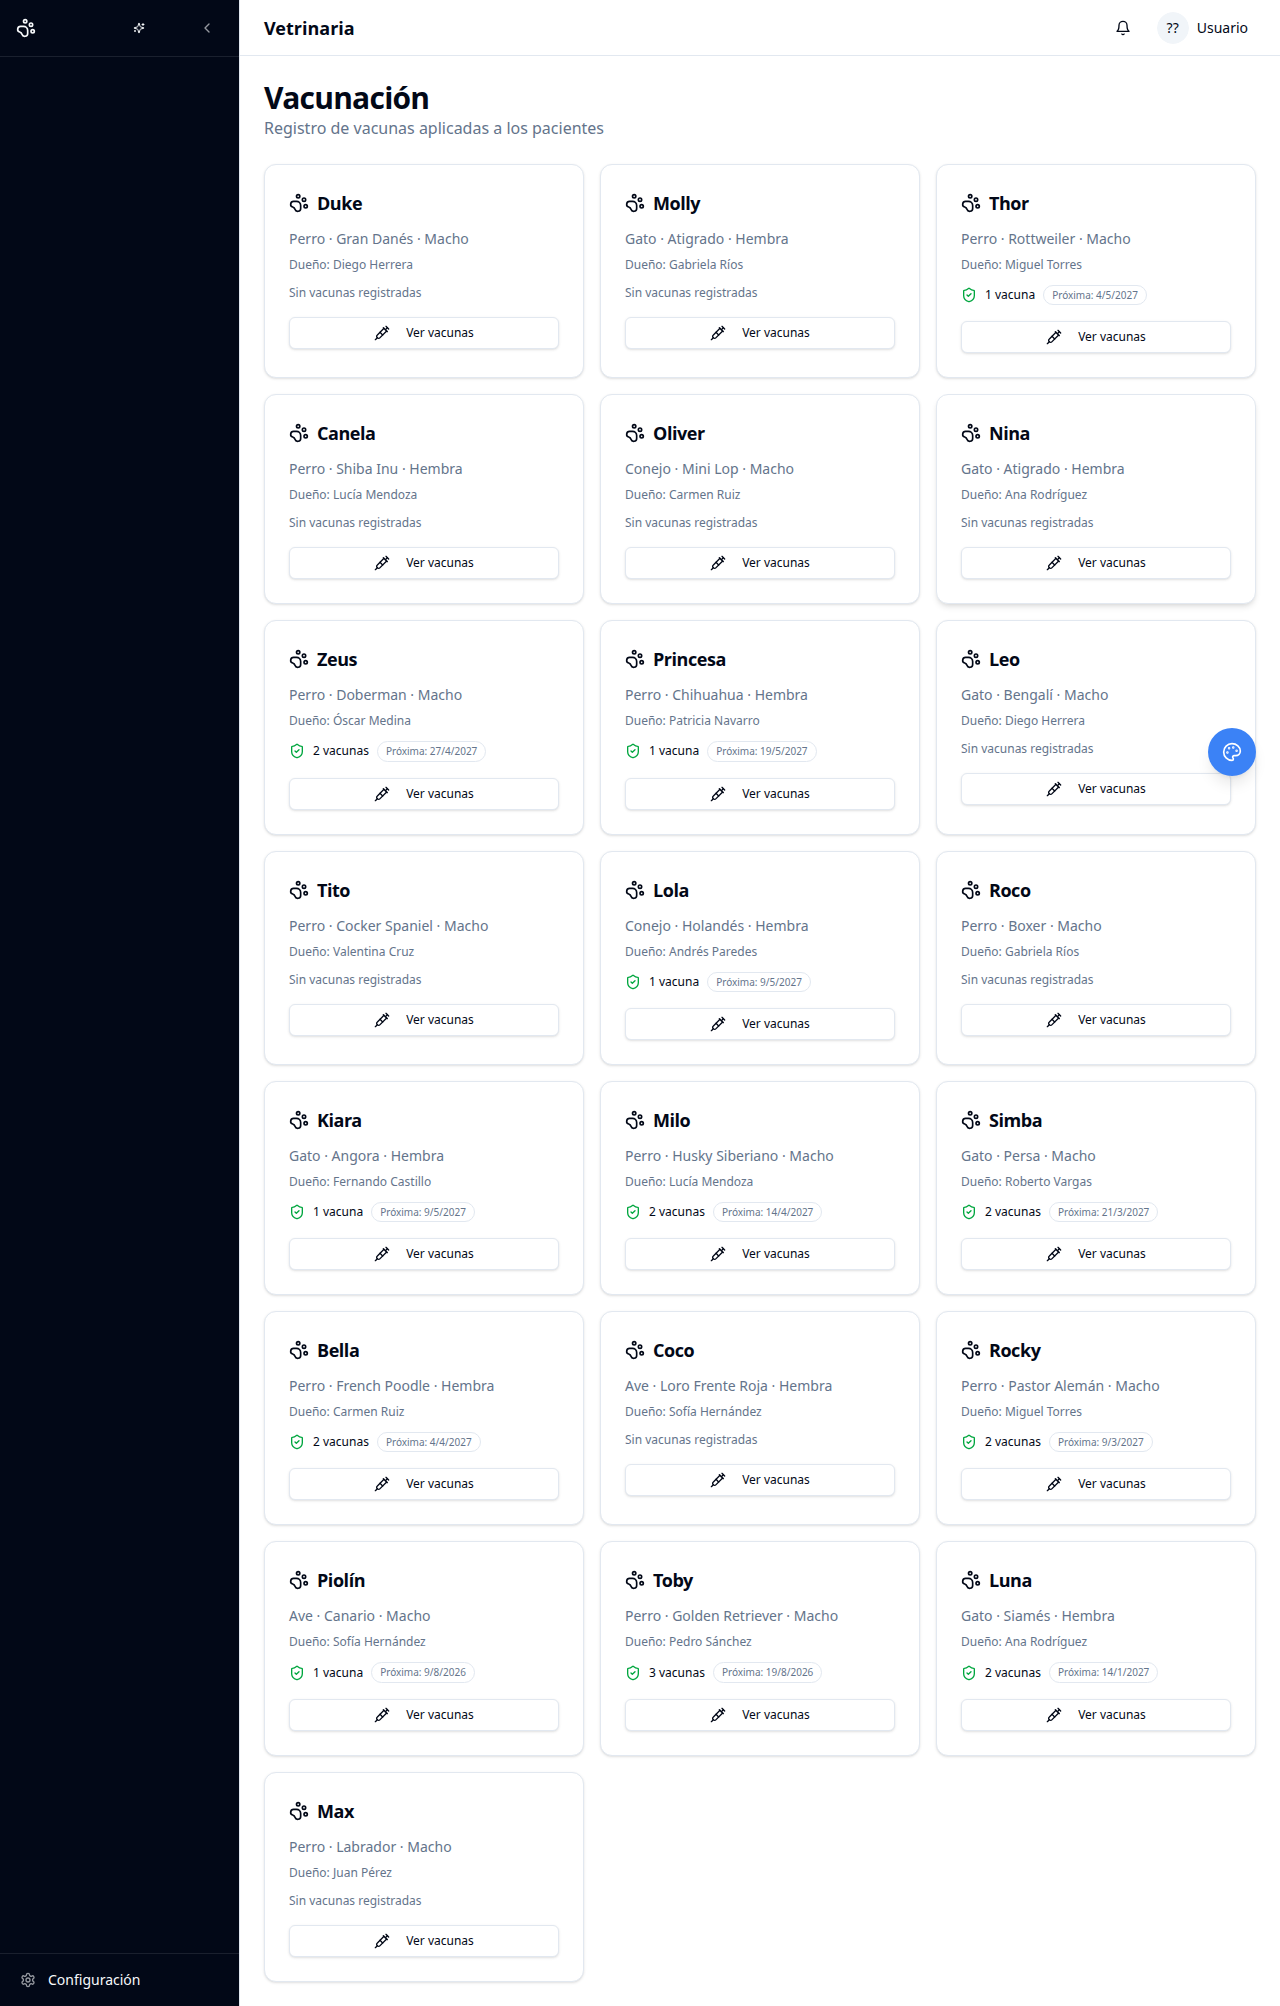
\includegraphics[width=\textwidth]{img/vet-vaccinations.png}
    \caption{Vista de resumen de vacunacion por paciente}
    \label{fig:vacunacion}
\end{figure}
